\begin{frame}{Introduction}
    Context:
    \begin{itemize}
        \item Collaboration with the Interaction- and Communication-
        based Systems research group at the University of St.\ Gallen
        \begin{itemize}
            \item \emph{IntellIoT} European project
            \item Multi-Agent Systems (MAS) applied to IoT
        \end{itemize}
    \end{itemize}
    \vspace{1cm}
    Result:
    \begin{itemize}
        \item Development of a tool that domain experts can use to
        intuitively design MAS organizations
    \end{itemize}
\end{frame}

\section{Context}
\subsection{The \textit{IntellIoT} Project}

\begin{frame}{The \textit{IntellIoT} Project}
    \begin{block}{The Next Generation IoT}
        IntellIoT is a Pan-European project focused on developing integrated, distributed, human-centered, and trustworthy IoT frameworks
    \end{block}

    \begin{columns}
        \begin{column}{0.45\textwidth}
            \begin{itemize}
                \item One of the project's missions is to enable \textbf{domain experts} to define complex systems intuitively
            \end{itemize}
        \end{column}
        \begin{column}{0.55\textwidth}
            \begin{figure}
                \centering
                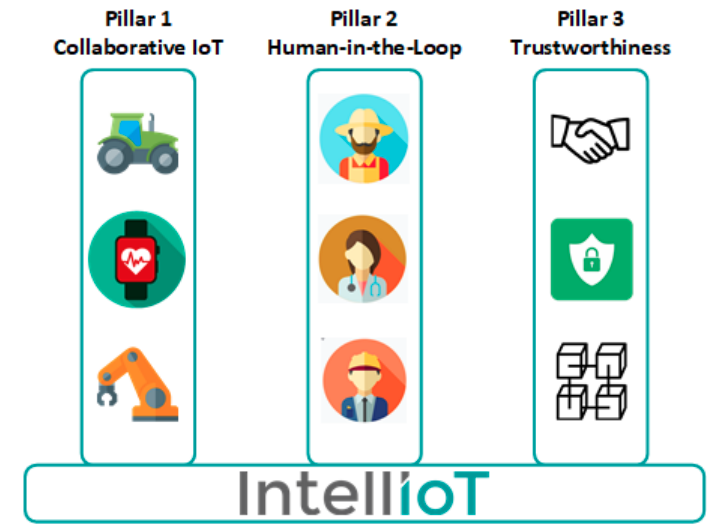
\includegraphics[width=0.8\textwidth]{images/intelliot-pillars.png}
            \end{figure}
        \end{column}
    \end{columns}
\end{frame}